\documentclass[12pt, a4paper]{article}
% Packages
\usepackage{fullpage}			% fullpage margins
\usepackage{graphicx, float}		% for graphics/figures
\usepackage{amsmath, amssymb}	% math formatting and symbols
\usepackage{color}
\usepackage{hyperref, footnote, url}
\usepackage{enumerate}
\usepackage{parskip}

% Environment for theorems
\usepackage{amsthm}			% http://www.ctex.org/documents/packages/math/amsthdoc.pdf
\newtheorem{lem}{Lemma}

\begin{document}
% Title
\title{CS3236 Project Report\\  Maximum Entropy }
\author{Xiang Pan \\ A0213836E \\ \texttt{xiangpan.cs@gmail.com}}
\date{04/09/2020} % Blank out the date
\maketitle


% Begin content
\section{Introduction}
This project is about maximum entropy. Firstly, we demonstrated the definition of the maximum entropy distribution and the maximum entropy principle. Then, we introduced applications of maximum entropy principle. Finally, we give an implementation of maximum entropy model and analyzed the result.



\section{Maximum Entropy Principle}
\subsection{A Simple Example}
In daily life, many things happen to show certain randomness, the results of the experiment are often uncertain, and we don't know the probability distribution that this random phenomenon obeys. Using some observed test samples or sample characteristics, how to
make a reasonable inference without a prior distribution?
For the simplest example(also the most used example), when we are asked what the probability of the dice showing 6 when we randomly throw a dice, we usually say 1/6. So why we can give such an answer? Just as stated above, we do not know the probability distribution of dice, we do not know any prior knowledge of such a probability system. Actually, we get the intuitive result with the usage of maximum entropy without notice.

\subsection{General Understanding}
The simplest way to illustrate maximum entropy principle is 'Model all that is known and assume nothing about that which is unknown'.

We know that entropy actually defines an uncertain when the entropy is the largest, it means that the random variable is the most uncertain, in other words, the random variable is the most random, and its behavior is accurate
Prediction is the most difficult. In this sense, the essence of the principle of maximum entropy is that, given the knowledge of some knowledge, about
The most reasonable inference for an unknown distribution is the most uncertain or random inference that fits known knowledge. This is the only reason we can make an unbiased choice, any other choice means that we add other constraints and assumptions, these constraints and falsely
suppose which cannot be made based on the information we have. 


\section{Maximum Entropy Distribution}

\subsection{Definition}
Formulaly, we have the entropy
\begin{equation}
H(X)=-\sum_{x\epsilon X}^{ }p(x)lgp(x)
\end{equation}


And the objective function of maximum entropy distribution is:
\begin{equation}
max(p\epsilon P)H(X)=-\sum_{(x)}^{ }p(y)logp(x)\label{MED}
\end{equation}
where the $P=\{p|p \in the \; distributions \; satisfiy \;the \;constraints\}$



\subsection{Solution}
We need to find the optimized the distribution $p$ (or $f$ demonstrated in Thomas Cover book \cite{10.5555/1146355}). 
We can use Lagrange multiplier because the differential entropy $h(p)$is a concave function over a convex set. (The book choose the continuous form, thus we choose the discrete form)

\subsubsection{Solution Example}
For a general example, we do not have additional constraints and we choose the discrete form. Thus the only constraint is:

\begin{equation}
	g(p_1,p_2,...,p_n)=\sum_{i=1}^{n}p_i=1
\end{equation}

\begin{equation}
F(p_1,p_2,...,p_n)=h(p_1,p_2,...,p_n)+\lambda *(g(p_1,p_2,...,p_n)-1) 
\end{equation}

We can do deviation for every $p_i$:
\begin{equation}
	\frac{\partial}{\partial p_{i}}\left(-\sum_{i=1}^{n} p_{i} \log _{2} p_{i}+\lambda\left(\sum_{i=1}^{n} p_{i}-1\right)\right)=0
	\end{equation}
we can get
\begin{equation}
	-\left(\frac{1}{\ln 2}+\log _{2} p_{i}\right)+\lambda=0
	\end{equation}


\begin{equation}
	p_{i}=\frac{1}{n}
\end{equation}

The result shows when there is no additional constraint, the average distribution is the maximum entropy distribution for discrete form. Such a result can also answer the mice question above.



\subsubsection{The proof of maximum}
In the Thomas Cover Book, they form a optimization problem, and a solution, Then proof the solution is indeed the maximum entropy distribution. We can use the information inequality below to prove the optimization.

\begin{equation}
	0 \leq D\left(p \| p^{*}\right)=-h(p)+h\left(p^{*}\right)
\end{equation}
Where $p^{*}$ is the result.

For the Lagrange multiplier one, it is harder to generalize but it directly solves the maximum entropy objective function. (It is just another expression of the calculus method in the book, but it may be more directly)




\subsection{Trivial case only with the constraint of entropy}

Every probability distribution is trivially a maximum entropy probability distribution under the constraint that the distribution has its own entropy. 

To proof this, rewire the $p(x)$
\begin{equation}
p(x)=\exp {(\ln {p(x)})}
\end{equation}
For the continuous situation,by choosing the $\ln {p(x)}\rightarrow f(x)$, we can get
\begin{equation}
\int \exp {(f(x))}f(x)dx=-H
\end{equation}


\subsection{With Constraints Case}
In a similar way, we can do the Lagrange multiplier for continuous form, such a process is also demonstrated in the Thomas Cover Book.

For different constraints, we can get different maximum entropy distribution. We only need to change the Lagrange multiplier part and do the optimization.




\subsection{Cases Examples}
We only show the most common case of constraints. Those maximum entropy distribution can get from the above process.


\subsubsection{Discrete Distribution}
\begin{table}[H]
\centering
\begin{tabular}{|c|c|}
\hline
Maximum Entropy Constraint & Maximum Entropy Distribution\\
\hline
Given Interval & Uniform Distribution\\
Given Mean & Uniform Distribution\\
Given Interval and standard deviation (variance) & Normal Distribution\\
$\mathbf{E}(x)=\mu, f \in \mathbf{n}-$ generalized binomial distribution&$f(k)=\left(\begin{array}{l}n \\ k\end{array}\right) p^{k}(1-p)^{n-k}$\\

$\mathbf{E}(x)=\lambda, f \in \infty$ -generalized binomial distribution& $f(k)=\frac{\lambda^{k} \exp (-\lambda)}{k !}
$\\




\hline
\end{tabular}
\end{table}

\subsubsection{Constraints Distribution}
\begin{table}[H]
\centering
\begin{tabular}{|c|c|}
\hline
Maximum Entropy Constraint & Maximum Entropy Distribution\\
\hline

$\mathrm{E}(x)=\frac{1}{\lambda}$&$f(x)=\lambda \exp (-\lambda x)$\\
$\mathbf{E}(x)=\mu, \mathbf{E}\left((x-\mu)^{2}\right)=\sigma^{2}$&$f(x)=\frac{1}{\sqrt{2 \pi \sigma^{2}}} \exp \left(-\frac{(x-\mu)^{2}}{2 \sigma^{2}}\right)$\\
$\mathbf{E}(\ln (x))=\psi(\alpha)-\psi(\alpha+\beta)$
$\mathbf{E}(\ln (1-x))=\psi(\beta)-\psi(\alpha+\beta)$&$f(x)=\frac{x^{\alpha-1}(1-x)^{\beta-1}}{B(\alpha, \beta)}$ for $0 \leq x \leq 1$\\
% Given Interval & Uniform Distribution\\
% Given Mean & Uniform Distribution\\
% Given Interval and standard deviation (variance) & Normal Distribution\\
\hline
\end{tabular}
\end{table}






% \begin{figure}[h]
% 	\centering
% 	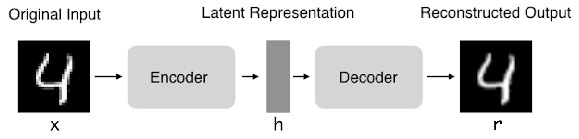
\includegraphics[width=0.7\linewidth]{./image/encoder-decoder.jpg}
% 	\caption{Encoder-Decoder Framework}
%   \label{encoder_decoder_image}
% \end{figure}







\section{Applications}
There are usually four applications using the principle of maximum entropy\cite{wiki:Principle_of_maximum_entropy} to inferential problems:
\begin{enumerate}[(i)]
\item Prior Probabilities(Naive Bayes)
\item Posterior Probabilities
\item Maximum Entropy Models
\item Probability Density Estimation
\item Maximum Entropy on Markov Chain
\end{enumerate}



\subsection{Maximum Entropy Models}
For Maximum Entropy Models \cite{10.5555/971143}, we can modify the equation \ref{MED} to conditional one to present the dependency between input and output:
\begin{equation}
max(p\epsilon P)H(Y|X)=-\sum_{(x,y)}^{ }p(x,y)logp(y|x)
\end{equation}

\begin{equation}
H(p) = -\sum_{x,y}\tilde p(x)p(y|x) \log p(y |x ) 
\end{equation}

Similarly, n optimization can be formulated as

\begin{equation}
	\begin{array}{ll}
	\max _{p \in P} & H(p)=-\sum_{x, y} \tilde{p}(x) p(y | x) \log p(y | x) \\
	\text { s.t. } & E_{p}\left(f_{i}\right)=E_{\tilde{p}}\left(f_{i}\right), \quad i=1,2, \cdots, d \\
	& \sum_{y} p(y | x)=1
	\end{array}
\end{equation}


The using Lagrange multiplier: 
\begin{equation}
L(p, \lambda) =\sum_{x,y}\tilde p(x)p(y|x) \log p(y |x )+\lambda_0(1 – \sum_y p(y|x) )+\sum_{i=1}^d \\
 \lambda_i \left(\sum_{x,y} \tilde p(x, y) f_i(x, y) – \sum_{x,y}\tilde p(x)p(y|x)f_i(x, y) \right) 
\end{equation}

Then, do the partial derivative:
\begin{equation}
	\begin{aligned}
	\frac{\partial L(p, \lambda)}{\partial p(y | x)} &=\sum_{x, y} \tilde{p}(x)(\log p(y | x)+1)-\sum_{y} \lambda_{0}-\sum_{i=1}^{d} \lambda_{i}\left(\sum_{x, y} \tilde{p}(x) f_{i}(x, y)\right) \\
	&=\sum_{x, y} \tilde{p}(x)(\log p(y | x)+1)-\sum_{x} \tilde{p}(x) \sum_{y} \lambda_{0}-\sum_{x, y} \tilde{p}(x) \sum_{i=1}^{d} \lambda_{i} f_{i}(x, y) \\
	&=\sum_{x, y} \tilde{p}(x)(\log p(y | x)+1)-\sum_{x, y} \tilde{p}(x) \lambda_{0}-\sum_{x, y} \tilde{p}(x) \sum_{i=1}^{d} \lambda_{i} f_{i}(x, y) \\
	&=\sum_{x, y} \tilde{p}(x)\left(\log p(y | x)+1-\lambda_{0}-\sum_{i=1}^{d} \lambda_{i} f_{i}(x, y)\right)
	\end{aligned}
\end{equation}





Then the extremum can be got when the partial derivative equals zero.

We can get the:
\begin{equation}
p_\lambda = p(y|x) = \frac{1}{Z_\lambda(x)}e^{\sum_{i=1}^d \lambda_if_i(x, y)} \\ 
where,Z_\lambda(x) =\sum_y e^{\sum_{i=1}^d \lambda_if_i(x, y) } 
\end{equation}


This $p_\lambda$ is the solution of the maximum entropy model, which has an exponential form, $f_i(x,y)$ is the feature function, $\lambda_i$ is the weight of the feature, the larger the $\lambda_i$, the more important the feature. 

Through such a process, we can accomplish the feature selection.

We have a solution, then just need to maximize the 
objective function:
\begin{equation}
	\begin{aligned}
\psi(\lambda) &=\sum_{x, y} \tilde{p}(x) p_{\lambda} \log p_{\lambda}+\sum_{i=1}^{d} \lambda_{i}\left(\sum_{x, y} \tilde{p}(x, y) f_{i}(x, y)-\sum_{x, y} \tilde{p}(x) p_{\lambda} f_{i}(x, y)\right) \\
&=\sum_{x, y} \tilde{p}(x, y) \sum_{i=1}^{d} \lambda_{i} f_{i}(x, y)+\sum_{x, y} \tilde{p}(x) p_{\lambda}\left(\log p_{\lambda}-\sum_{i=1}^{d} \lambda_{i} f_{i}(x, y)\right) \\
&=\sum_{x, y} \tilde{p}(x, y) \sum_{i=1}^{d} \lambda_{i} f_{i}(x, y)-\sum_{x, y} \tilde{p}(x) p_{\lambda} \log Z_{\lambda}(x) \\
&=\sum_{x, y} \tilde{p}(x, y) \sum_{i=1}^{d} \lambda_{i} f_{i}(x, y)-\sum_{x} \tilde{p}(x) \log Z_{\lambda}(x)
\end{aligned}
\end{equation}

The Maximum Entropy's solution contains the exponent
form. In fact, such a form can be expressed uniformly in exponential families of distributions.


\subsection{Burg's Maximum Entropy Theorem}
\subsubsection{Max Entropy Rate Stochastic processes}

\begin{equation}
\begin{aligned}
H\left(X_{1}, \ldots, X_{n}\right)=
\sum_{i=1}^{n} H\left(X_{i} | X_{i-1} \ldots X_{1}\right)
\\\leq 
\sum_{i=1}^{n} H\left(X_{i}\right) 
=n H(X) 
\end{aligned}
\end{equation}

For a stochastic process with arbitrary dependencies, we have: 
\begin{equation}
	H(\mathcal{X}):=\lim _{n \rightarrow \infty} \frac{H\left(X_{1}, \ldots, X_{n}\right)}{n}
\end{equation}
Every symbols' entropy is limited, thus we have :  
\begin{equation}
	H^{\prime}(\mathcal{X}):=\lim _{n \rightarrow \infty} H\left(X_{n} | X_{n-1}, \ldots, X_{1}\right)
\end{equation}\label{limit_entropy}

Stationary stochastic process: satisfy the shift properties:  
\begin{equation}
	\begin{aligned}
	&p\left(X_{1}, \ldots, X_{n}\right)=p\left(X_{1+l}, \ldots, X_{n+l}\right)\\
	&\forall n 
\end{aligned}
\end{equation}\label{shift}

Combine the \ref{limit_entropy} and \ref{shift}, we can formulate the first order Markov process:
\begin{equation}
	H(\mathcal{X})=\lim _{n \rightarrow \infty} H\left(X_{n} | X_{n-1}\right)=H\left(X_{2} | X_{1}\right)
\end{equation}


Then, for the max entropy rate stochastic process with the constraints:

\begin{equation}
	E\left[X_{i} X_{i+k}\right]=\alpha_{k} \quad \text { for } k=0,1 \ldots p \quad \forall i
\end{equation}
We can formulate the whole process as :  
\begin{equation}
	X_{i}=-\sum_{i=1}^{p} a_{k} X_{i-k}+Z_{i} \quad Z_{i} \stackrel{i i d}{\sim} \mathcal{N}\left(0, \sigma^{2}\right)
\end{equation}

\subsubsection{Proof}
We can use the chain rule to get the upper bound of $H\left(X_{1}, \ldots, X_{n}\right)$ to prove the process formula:
\begin{equation}
	\begin{aligned}
	% &\begin{aligned}
	H\left(X_{1}, \ldots, X_{n}\right) & \leq H\left(Z_{1}, \ldots, Z_{n}\right) \\
	&=H\left(Z_{1}, \ldots, Z_{p}\right)+\sum_{i=p+1}^{n} H\left(Z_{i} | Z_{i-1}, \ldots, Z_{1}\right) \text { (chain rule) }\\
	% \end{aligned}\\
	&\leq H\left(Z_{1}, \ldots, Z_{p}\right)+\sum_{i=p+1}^{n} H\left(Z_{i} | Z_{i-1}, \ldots, Z_{i-p}\right) \text { (conditioning doesn't increase entropy) }\\
	&=H\left(Z_{1}^{\prime}, \ldots, Z_{p}^{\prime}\right)+\sum_{i=p+1}^{n} H\left(Z_{i}^{\prime} | Z_{i-1}^{\prime}, \ldots, Z_{i-p}^{\prime}\right)\\
	&=H\left(Z_{1}^{\prime}, \ldots, Z_{n}^{\prime}\right)
	\end{aligned}
\end{equation}

We can also check the form satisfied the constraint by using Yule-Walker equations.

\subsubsection{Application of Maximum Entropy on Markov Model(MEMM)}
Just as the maximum entropy model is the application of the maximum entropy principle in a single variable. The MEMM \cite{mccallum2000maximum} is the application of maximum entropy theory on Markov Chain related to arbitrary dependent variables' sequence.

We can also modify the formula to conditioning one, where x is the observed value, and y is the label of the sequence.  In other words, the X is the observed distribution, the Y is the true distribution. We need to inference the true distribution from what we observed.
\begin{equation}
P\left(y_{1}, \ldots, y_{n} | x_{1}, \ldots, x_{n}\right)=\prod_{t=1}^{n} P\left(y_{t} | y_{t-1}, x_{t}\right)
\end{equation}


\begin{equation}
	P\left(y | y^{\prime}, x\right)=P_{y^{\prime}}(y | x)=\frac{1}{Z\left(x, y^{\prime}\right)} \exp \left(\sum_{a} \lambda_{a} f_{a}(x, y)\right)
\end{equation}

Here, the $f$ is the feature function, and the $\lambda$ is the feature weight. The $f$ can be seen as the connection measure between input and output. Those can give the more entropy will give more weight. Similarly, such a process can be seen as a feature selection.




% since conditioning does not increase entropy 



\section{Experiments of the Maximum Entropy Model}
\subsection{Task}
For the Maximum Entropy Model, we want to find a suitable input-output transformation function. For the $x$ as the input data or feature. $y$ as the label for optimization. Specifically, We do the sentiment classification based on Maximum Entropy Model Classifier. Thus the $x$ is the text feature, and $y$ is the classification label.
\subsection{Dataset}
We use the nltk movie reviews dataset, we changed the training samples' number to analyze the learning ability of Maximum Entropy on Model.

\subsection{Optimization}
The objective function is without an analytical solution, however, the objective function is always convex function. Hence, we can use convex optimization methods to get the final solution. 

\subsection{Results}
\begin{figure}[h]
	\centering
	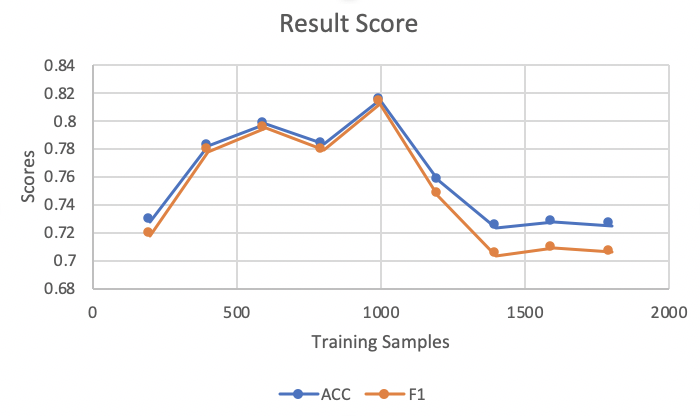
\includegraphics[width=0.7\linewidth]{./image/result.jpg}
	\caption{The Maximum Entropy Model Results}
  \label{results}
\end{figure}



\subsection{Analysis}

\subsubsection{Pros}
\begin{enumerate}[(i)]
	\item Only needs to concentrate on selecting features, without spending effort consider how to use these features.  
	\item Generally does not require the independent assumptions often used in other methods of modeling.
	\item Slippage can be considered through feature selection, without the need to consider it separately using conventional smoothing algorithms.
	\item The contribution of the probability distribution is determined by the parameters, which can be obtained by iterative training by a certain algorithm.
	\item The constraints can be set flexibly, and the degree of constraints can adjust the model's adaptability to unknown data and the degree of fitting to known data
	\end{enumerate} 
\subsubsection{Cons}
The relationship between the number of constraint functions and the number of samples leads to high time complexity.


\section{Conclusion}
In this report, we demonstrate the Maximum Entropy Principle and analyzed its various forms in discrete, continuous variable and variable sequence on Markov Chains. Furthermore, we give a detailed formal definition and formula derivation in its application- Maximum Entropy Model and Maximum Entropy Markov Model. Finally, we implemented a test case of Maximum Entropy Model on the movie review dataset, analyzed the result and learning ability of Maximum Entropy Model. In addition, we provide the pros and cons of the MEM algorithm. 


\newpage
\bibliographystyle{unsrt}
\addcontentsline{toc}{section}{References}
\bibliography{Ref}



\end{document}